\documentclass[12pt, a4paper,twoside]{report}
\usepackage{amsmath,amsthm,verbatim,amssymb,amsfonts,amscd,color,graphicx,subcaption}
\usepackage{graphics,tikz,pgflibraryarrows,pgflibrarysnakes,booktabs,multirow}
\usepackage{hyperref,setspace} %hypersetup used for the link colors, say the contents, the bibliography, and the cited text numbering.
\hypersetup{colorlinks=true,linkcolor=black,citecolor=magenta,urlcolor=cyan,pdftitle={Sharelatex Example},bookmarks=true,} %links colors
\usepackage{blindtext,scrextend}
\addtokomafont{labelinglabel}
{\rmfamily\mdseries}

\usepackage{algpseudocode,algorithm,algorithmicx}
\newcommand*\DNA{\textsc{dna}}
\newcommand*\Let[2]{\State #1 $\gets$ #2}
\algrenewcommand\algorithmicrequire{\textbf{Precondition:}}
\algrenewcommand\algorithmicensure{\textbf{Postcondition:}}
\usepackage{enumitem}
\newlist{Description}{description}{2}
\setlist[Description]{style=nextline}
\SetEnumitemKey{margin}{leftmargin={\widthof{#1}+2em}}

\usepackage[top=1.2in,bottom=1in,left=1 in,right=1in]{geometry} % setting for the pages margin
\DeclareMathOperator{\E}{\mathbb{E}}
\usepackage[utf8]{inputenc}
\usepackage[english]{babel}
\usepackage{fancyhdr}
\pagestyle{fancy}
\fancyhf{}
\fancyhead[LE,RO]{\rightmark} % heading for the page
\fancyfoot[CE,CO]{\thepage}   % heading for the page

\newtheoremstyle{mydef}% name
{12pt}% Space above
{12pt}% Space below
{}% Body font
{}% Indent amount
{\bfseries}% Theorem head font
{}% Punctuation after theorem head
{.9em}% Space after theorem head
{}% Theorem head spec (can be left empty, meaning `normal')
\newtheoremstyle{myplain}{12pt}{12pt}{\itshape}{}{\bfseries}{}{.9em}{}
\newtheoremstyle{mypro}{12pt}{12pt}{}{}{\bfseries}{}{.9em}{}
%\theoremstyle{def}
\theoremstyle{definition}
\newtheorem{definition}{Definition}[section]
\newtheorem*{example}{Example}
%\newtheorem{definition}[Theorem]{Definition} % definition numbers are dependent on theorem numbers
%\newtheorem{example}[Theorem]{Example} % same for example numbers

\theoremstyle{myplain}
\newtheorem{theorem}{Theorem}[section]
\newtheorem{corollary}[theorem]{Corollary}
\newtheorem{lemma}[theorem]{Lemma}
\theoremstyle{mypro}
\newtheorem{proposition}{Proposition}[section]
\newtheorem{remark}{Remark}[section]
\newtheorem*{remark*}{Remark} %For having unnumbered remarks. 
\newtheorem{pro}{Proposition}[section]
\newtheorem{theo}[pro]{Theorem}
%\renewcommand{\theremark}{\arabic{remark}}%\renewcommand\qedsymbol{$blacksquare$} %proof end color
\def\label#1{\@bsphack\protected@write\@auxout{}{\string\newlabel{#1}{{\@currentlabel}{\thepage}}}\@esphack} 
\def\QEDmark{\ensuremath{\square}}
\def\proof{\paragraph{Proof:}}
\def\endproof{\hfill\QEDmark}

\begin{document}
%--------------------------------------Start of Title Page-------------------------------------
\begin{titlepage}
\begin{center}
\vspace*{.03\textheight}
{\scshape\LARGE The University of Melbourne\par}\vspace{0.6cm}
\textsc{\Large Department of Mathematics and Statistics}\\[0.9cm]
\rule{0.95\textwidth}{1.2 pt}\vspace{0.3cm}\\
{\huge \textbf{Population History Estimation:\\ A Coalescent Theory Approach}\par}\vspace{0.3cm} % Thesis title
\rule{0.95\textwidth}{1.2 pt}
\vfill
\vspace{0.6cm}

\begin{minipage}[t]{0.4\textwidth}
\begin{flushleft} \large
\emph{Author:}\\
{Xuehua \textsc{Lan}}
\end{flushleft}
\end{minipage}
\begin{minipage}[t]{0.4\textwidth}
\begin{flushright} \large
\emph{Supervisor:} \\
{Nathan \textsc{Ross}}
\end{flushright}
\end{minipage}\\[3cm]

\vfill
\vspace*{.24\textheight}
\large \textit{A thesis submitted in partial fulfillment of the requirements\\ for the degree of Master of Science}\\[0.6cm] 
\vfill
\vspace*{.12\textheight}

{\large May~2017}\\[4cm]
\end{center}
\end{titlepage}
%--------------------------------------End of Title Page-------------------------------------

\thispagestyle{empty}
\vspace*{.36\textheight}
\begin{center}
\textit{Dedicated to all my teachers\\ and \\to my parents.}
\end{center}
\clearpage

\renewcommand{\abstractname}{Acknowledgments}
\begin{abstract}
My foremost gratitude goes to my supervisor, Nathan Ross.
\end{abstract}



\pagenumbering{Roman}
\tableofcontents

\listoffigures

\chapter*{List of Notations}
%\section*{Nomenclature}
\begin{labeling}{alligator}
\item [$\mathbb{R}$] real number.
\item [$\lfloor x \rfloor$] the biggest integer less or equal to x.
\item [$\lceil x \rceil$] the smallest integer greater or equal to x.
\item [$\textbf{1}_{\{\cdot\}}$] indicator function.
\item [$\mathcal{D}:=(\mathcal{D},d)$] pseudo-metric or metric space of set $\mathcal{D}$ with metric d.
\item [$(\Omega, \mathcal{F}, \textbf{P})$] probability space, where $\mathcal{P}$ is a family of probability measure, and $\mathcal{F}$ is a $\sigma$-algebra.
\item [$co(\mathcal{P})$] the convex hull of $\mathcal{P}$. 
\item [$\mathbb{E}(\cdot)$] expectation of the interest.
\item [$\theta(P)$] parameter of interest with values in $(\mathcal{D},d)$.
\item [$\hat{\theta}=\hat{\theta}(X)$] an estimator of $\theta(P)$ based on an X with distribution P.
\item [$d_{TV}(P, Q)$] the total variation distance between P and Q.
\item [$d_{H}(P,Q)$] the Hellinger distance between P and Q.
\item [$d_{KL}(P||Q)$] the Kullback Leibler distance from Q to P, also known as relative entropy.
\end{labeling}

\chapter*{List of Abbreviations}
\begin{labeling}{alligator}
\item [RVs] Random variables
\item [SNP] Single Nucleotide Polymorphism
\item [MRCA] Most Recent Common Ancestor
\item [WF] Wright-Fisher, refer to a coalescent model
\item [KL] Kullback-Leibler, refer to a statistical distance
\item [AFS] Allele frequency spectrum, some may refer as site frequency spectrum
\item [SFS] Sample frequency spectrum
%\item [CG] Completed 
\item [AG] Ancient genealogy
\item [TG] Truncated genealogy
\end{labeling}

\clearpage

%\setcounter{page}{1}
%\pagestyle{plain}
\pagenumbering{arabic} % using a different page conting methods to distinguish between the front pages
\chapter*{Preface} % the '*' avoid the Preface being numbered in the contents
\addcontentsline{toc}{chapter}{\protect\numberline{}Preface}
This presented thesis is the research project of the Master of Science degree. In this thesis, the error of estimating the population history on a coalescent inference approach will be presented.\\

Coalescent theory is one tool in theoretical population genetics to mathematically model the process of evolution, it is a stochastic process that describes the probability distribution on ancestors at the genetic levels and formulates the genetic drift backwards in time. Along the process, one can reconstruct past genealogy from present day genetic data. Given a past population shape, the distributions of times of coalescence and the expected sample frequency spectrum (SFS) can be used to infer this history. In this thesis, we look at the statistical error made when using these two methods for inference. First we derive bounds on the error made in the setting of populations with a bottleneck, in terms of the amount of data used. We then expand our interests to population shapes that have split from one population, constructing the density of coalescent times and then the distribution of expected SFS. Finally we use these derivations to obtain bounds on the error when using these two methods for inference, again in terms of the amount of data used.\\

This thesis consists of 6 chapters. Firstly, we introduce the developments in coalescent theory in chapter 1. Chapter 2 is devoted to prior knowledge in metrics and functions, probability theory, information theory, minimax theory, and coalescent theory. Then in chapter 3 some useful techniques and results that can help us to derived outcomes in chapter 4 will be explored. Although this chapter focuses on inferring in a single population, there are broader insights one can gained for further inference between multiple populations. We start looking at the population history estimation in chapter 4 and focus in a single population in this chapter. Two developed methods will be explored to construct the distributions that can reveal the population size functions, based on these two methods, we derived minimax bounds and compared in terms of the amount of data. In chapter 5, we turn our interests to population shapes that have split from one population, which is also known as diverging populations. In terms of two distribution methods explored in chapter 4, we construct these two distributions with respect to a diverging population, and output a minimax lower bounds between distributions for comparison. A general conclusion will be given in chapter 6, with a discussion on strengths and limitations.

\clearpage

%--------------------------------------------------------------------------------------------------------------------------------
%                                                                 Introduction
%--------------------------------------------------------------------------------------------------------------------------------
\chapter{Introductions}
In this first chapter, we introduced the developments in coalescent processes.\\

We firstly introduced the Kingman coalescent, and briefly look at the drift of gene itself, to other forces varies the processes, such as mutation, recombination, and flows of population. Along with discussing the limitations of Kingman coalescent, other types of coalescent will be introduced.\\

One powerful strategy for extracting information from genetic data is to mathematically model the process of evolution. Theoretic population genetic was formed at the starts of the 20’s, half century after Darwin found the evolution of traits. In the processes on formulating the evolution of genomes with polymorphism data, the foundations are grounded on stochastic formalization by Fisher \cite{Fisher}, Wright \cite{Wright}, and Haldane \cite{Haldane} in 1930’s. Wright-Fisher is a cornerstone model in population genetics, with binary selection scheme underlies, it assuming in each generation at most one coalescent event happen to one pair of individual, with $2N$ haploid individuals, or $N$ diploid individuals. All individuals in each generation are considered to reproduced next generations and then die at the end of each generation.\\

Diffusion approach was firstly developed to capture the neutral net movements between genes in 1950. Not until 1982, Kingman \cite{Kingman} introduced the coalescent approach, this approach allow us to reconstruct the genealogy from present and relax preferred selection in the process.\\

Kingman coalescent rely on Wright-Fisher model and taking limits in continuous time, the coalescent process can be considered as a homogenous pure death processes start at $n$ lineages (states), see figure 1.1 for example, and eventually coalescent into $1$ lineages, which in coalescent theory known the most recent common ancestor (MRCA). The associated death rate in the each state is actually the frequency of the coalescent, and the statistics of the process can be formulated through the analysis of this frequency at each number of lineages (states). Under the binary coalescent setting as a pure death processes, the finite states (lineages) give advantages in inferences. Many existing results can be applied without consider conditional assumptions in the case of explosive continuous time process.\\

\begin{figure}[!h]
\label{Fig:Pure Death Process}
\begin{center}
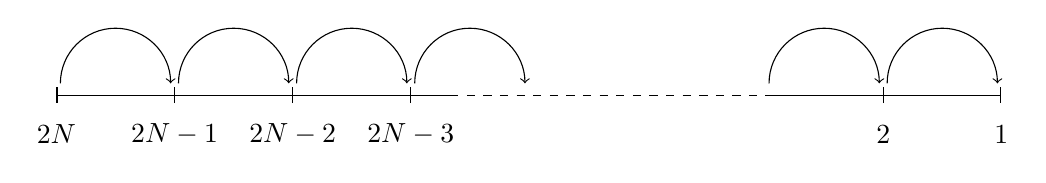
\begin{tikzpicture}
%picture
\draw [|-] (0,0)--(5,0);
\draw [dashed] (5,0)--(9,0);
\draw [-|] (9,0)--(12,0);
\draw (1.5,-0.1)--(1.5,0.1);
\draw (3,-0.1)--(3,0.1);
\draw (4.5,-0.1)--(4.5,0.1);
\draw (10.5,-0.1)--(10.5,0.1);
\node at (0,-0.5) {$2N$};
\node at (12,-0.5) {$1$};
\node at (1.5,-.5) {$2N-1$};
\node at (3,-.5) {$2N-2$};
\node at (4.5,-.5) {$2N-3$};
\node at (10.5,-.5) {$2$};
\draw[<-] (1.45,0.15) arc (0:180:0.7);
\draw[<-] (2.95,0.15) arc (0:180:0.7);
\draw[<-] (4.45,0.15) arc (0:180:0.7);
\draw[<-] (5.95,0.15) arc (0:180:0.7);
\draw[<-] (10.45,0.15) arc (0:180:0.7);
\draw[<-] (11.95,0.15) arc (0:180:0.7);
\end{tikzpicture}
\end{center}
\caption{A pure death process for Kingman coalescent.}
\end{figure}

Wright-Fisher model is not the only model to approach the Kingman coalescent, it can also be approached by Moran model, introduced by Moran \cite{Moran} in 1958. Both Wright-Fisher and Moran model are discrete and all the individuals waiting to coalescent are considered random selected and so are exchangeable, which introduced a generalized discrete model, the Canning model. As two special cases of the Caning model, the main differences between them is that Moran model allows overlapping in generations while Wright-Fisher model is not, and consequently the coalescent time of Moran model is $1/2N$ ($1/N$) slower than WF model in haploid (diploid) individuals.\\
%Given finite number of samples, and using the mathematical evolution models to find the most recent common ancestor (MRCA), can be seen as a Markov chain,

The models mentioned above are basic formulations of individuals' births and deaths, there are other forces along with the drift. Mutations are considered as one of the important forces of the coalescent processes, which occur occasionally in the processes by changing the gene information. To mimic the processes, infinite alleles models and infinite sites models are developed. These two models are based on different accessible genetic information, on the alleles and the segregating sites respectively. Infinite alleles models create a new allele in each mutation, so one should count number of alleles types and number of presentations. Mathematical proof shows the number of allele types converges in a reciprocal logarithm, but it is sufficient to provide all the information. Infinite sites model, on the other hand, mutation affects a site that was previously unaffected before, with only two bound nucleotides (adenine (A) paired with thymine (T), and guanine (G) paired with cytosine (C)), one can tells the mutant genes under infinite site setting.\\

There are other intrinsic forces such as recombination and natural selections. Not all these forces are mutually happen, in fact, in reality, allele have higher possibility to happen in neighborhood regions; and there are some loci are considered to have higher mutant rate than others, which are known as hot spot.\\

Extrinsic forces like population flows due to wars and diseases, industrial revolutions and economic booms, and migration are also factors that affect the drift of the coalescent processes, Kingman coalescent allows us to relax these forces in it.\\

Coalescent theory allow us to track back past genealogies, the applications of coalescent can be widely used as disease gene mapping, given that the distribution can be constructed on the ancestor of a group of sample genes, one can calculate the distributions of forces like mutations and recombination, to calculated the theoretical proof of the processes. It gives theoretic heterozygous of the population.\\

Readers may find our works mainly based on Kingman coalescent with Wright-Fisher model underlies, but should also note the limitations based on it. In addition that population N large enough, Kingman coalescent requires the number of offspring produced by each parent is small compared to the population size $N$ in order to satisfies small fluctuation. Furthermore, Kingman coalescent limits on the binary setting, for each pair to coalescent in each generation. In this setting, violations exist in real life application, to tackle this, multiple merger of one coalescent with two or more lineages are introduced. See figure 1.2 for motivation.\\

\begin{figure}[!h]
\begin{center}
\begin{tikzpicture}
%picture
\draw [|-] (0,0)--(5,0);
\draw [dashed] (5,0)--(9,0);
\draw [-|] (9,0)--(12,0);
\draw (1.5,-0.1)--(1.5,0.1);
\draw (3,-0.1)--(3,0.1);
\draw (4.5,-0.1)--(4.5,0.1);
\draw (10.5,-0.1)--(10.5,0.1);
\node at (0,-0.5) {$2N$};
\node at (12,-0.5) {$1$};
\node at (1.5,-.5) {$2N-1$};
\node at (3,-.5) {$2N-2$};
\node at (4.5,-.5) {$2N-3$};
\node at (10.5,-.5) {$2$};
\draw[<-] (4.45,0.3) arc (0:180:2.2);
\draw[<-] (5.95,0.3) arc (0:180:2.2);
\draw[<-] (9.05,0.3) arc (0:180:3.75);
\draw[<-] (10.45,0.3) arc (0:180:0.65);
\draw[<-] (11.95,0.3) arc (0:180:0.7);
\draw[<-] (2.95,0.3) arc (0:180:0.7);
\draw[<-] (11.95,0.3) arc (0:180:0.7);
\end{tikzpicture}
\end{center}
\caption{A pure death process for multiple merger coalescent.}
\end{figure}




%--------------------------------------------------------------------------------------------------------------------------------
%                                                                  Preliminaries
%--------------------------------------------------------------------------------------------------------------------------------
\chapter{Preliminaries}
This chapter is devoted to some mathematical facts, definitions and results in probability, information, and coalescence theory.


%--------------------------------------------------------------------------------------------------------------------------------

\appendix
\chapter{Supplement Notes and Proofs}
%\addcontentsline{toc}{chapter}{\protect\numberline{A}Appendix}
\pagenumbering{roman}
\section{Sets and Urn Models}

%--------------------------------------------------------------------------------------------------------------------------------
%                                                                    Bibliography
%--------------------------------------------------------------------------------------------------------------------------------
\begin{thebibliography}{10}
\addcontentsline{toc}{chapter}{\protect\numberline{B}Bibliography}
\bibitem[1]{Blum & Rosenberg}Blum, M, G, B., and Rosenberg, N, A. (2007). Estimating the Number of Ancestral Lineages Using a Maximum-Likelihood Method Based on Rejection Sampling. \textit{Genetics} \textbf{176} 3.
\bibitem[2]{Bhaskar & Song}Bhaskar, A., and Song, Y. S. (2014). Descartes' rule of signs and the identifiability of population demographic models from genomic variation data. \textit{Annals of Statistics} \textbf{42} 2469-2493.
\bibitem[3]{Chen}Chen, H. (2012). The joint allele frequency spectrum of multiple populations: A coalescent theory approach. \textit{Theoretical Population Biology} \textbf{81} 179-195.
\bibitem[4]{Cover & Thosmas}Cover, T, M., and Thomas, J, A. (1991) \textit{Elements of Information Theory}. first edition, Wiley New York.
\bibitem[5]{Durrett}Durrett, R. (2008). \textit{Probability Models for DNA Sequence Evolution}. second edition,  Springer New York.
\bibitem[6]{Fisher}Fisher, R, A. (1930). \textit{The Genetical Theory of Natural Selection}. second edition,  Clarendon Press, Oxford, UK.
\bibitem[7]{Griffiths & Tavare}Griffiths, R. C., amd Tavare, S. (1998). The age of mutation in the general coalescent tree. \textit{Stochastic Models} \textbf{14} 273-295.
\bibitem[8]{Haldane}Haldane, J, B, S. (1932). \textit{The causes of evolution}. Longmans, Green and Co., London.
\bibitem[9]{Kim et al.}Kim, J., Mossel, E., R$\acute{a}$cz, M. Z. and Ross, N. (2015). Can one hear the shape of a population history? \textit{Theoretical Population Biology} \textbf{100} 26-38.
\bibitem[10]{Kimura & Ohta}Kimura, M., and Ohta, T. (1973). The age of a neutral mutant persisting in a finete population. \textit{Genetics} \textbf{75} 199-212.
\bibitem[11]{Kingman}Kingman, J, F, C. (1982). The coalescent. \textit{Stochastic Processes and their Applications} \textbf{13} 235-248.
\bibitem[12]{LeCam}Le Cam, L. (1973). Convergence of estimates under dimensionality restrictions. \textit{Annuals of Statistics} \textbf{1} 38-53.
\bibitem[13]{Li & Durbin}Li, H., and Durbin, R. (2011). Inference of human population history from individual whole-genome sequences. \textit{Nature} \textbf{475} 493-496.
\bibitem[14]{Moran}Moran, P, A, P. (1958). Random processes in genetics. \textit{Mathematical Proceedings of the Cambridge Philosophical Society} \textbf{1} 60-71.
\bibitem[15]{Myers et al.}Myers, S., Fefferman, C., and Patterson, N. (2008) Can one learn history from the allelic spectrum? \textit{Theoretical Population Biology} \textbf{73(3)} 342-348.
\bibitem[16]{Polanski et al.}Polanski, A., Bobrowski, A., and Kimmel, M. (2003). A note on distributions of times to coalescence, under time-dependent population size. \textit{Theoretical Population Biology} \textbf{63} 33-40.
\bibitem[17]{Polanski & Kimmel}Polanski, A., and Kimmel, M. (2003). New Explicit Expressions for Relative Frequencies of Single-Nucleotide Polyorphisms with application to statistical inference on population growth. \textit{Genetics} \textbf{165} 427-436.
\bibitem[18]{Shannon}Shannon, C. E. (1948). A mathematical theory of communication. \textit{Bell system technical journal} \textbf{27} 379–423, 623–656.
\bibitem[19]{Sheehan et al.}Sheehan, S., harris, K., and Song, Y. S. (2013). Estimating variable effective population sizes from multiple genomes: A sequentially Markov conditional sampling distribution approach. \textit{Genome Research} \textbf{15} 1576-1583.
\bibitem[20]{Tavare}Tavar$\acute{e}$, S. (1984). Line-of-descent and genealogical processes, and their applications in population genetics models. \textit{Theoretical Population Biology} \textbf{26(2)} 119-164.
\bibitem[21]{Terhorst & Song}Terhorst, J., and Song, Y. S. (2015). Fundamental limits on the accuracy of demographic inference based on the sample frequency spectrum. \textit{Proceedings of the National Academy of Sciences of the United States of America} \textbf{112}(25) 7677-7682.
\bibitem[22]{Wright}Wright, S. (1931). Ecolution in Mendelian populations. \textit{Genetics} \textbf{16} 0097-0159.
\bibitem[23]{Yu}Yu, B. (1997). Assouad, Fano, and Le Cam. In D. Pollard, E. Torgersen, $\&$ G. L. Yang (Ed.), \textit{Festschrigt for Lucien Le  Cam} (pp. 423-435). Springer New York.
\end{thebibliography} 
%Lawrence, J. A., &  Dodds, A. E. (2003). Goal-directed activities and life-span development. In J. Valsiner & K. Connolly (Eds.), Handbook of developmental psychology (pp. 517-533). London, England: Sage Publications.

\end{document}